\documentclass[journal,12pt,twocolumn]{IEEEtran}

\usepackage{setspace}
\usepackage{gensymb}
\singlespacing
\usepackage[cmex10]{amsmath}

\usepackage{amsthm}

\usepackage{mathrsfs}
\usepackage{txfonts}
\usepackage{stfloats}
\usepackage{bm}
\usepackage{cite}
\usepackage{cases}
\usepackage{subfig}

\usepackage{longtable}
\usepackage{multirow}

\usepackage{enumitem}
\usepackage{mathtools}
\usepackage{steinmetz}
\usepackage{tikz}
\usepackage{circuitikz}
\usepackage{verbatim}
\usepackage{tfrupee}
\usepackage[breaklinks=true]{hyperref}
\usepackage{graphicx}
\usepackage{tkz-euclide}

\usetikzlibrary{calc,math}
\usepackage{listings}
    \usepackage{color}                                            %%
    \usepackage{array}                                            %%
    \usepackage{longtable}                                        %%
    \usepackage{calc}                                             %%
    \usepackage{multirow}                                         %%
    \usepackage{hhline}                                           %%
    \usepackage{ifthen}                                           %%
    \usepackage{lscape}     
\usepackage{multicol}
\usepackage{chngcntr}

\DeclareMathOperator*{\Res}{Res}

\renewcommand\thesection{\arabic{section}}
\renewcommand\thesubsection{\thesection.\arabic{subsection}}
\renewcommand\thesubsubsection{\thesubsection.\arabic{subsubsection}}

\renewcommand\thesectiondis{\arabic{section}}
\renewcommand\thesubsectiondis{\thesectiondis.\arabic{subsection}}
\renewcommand\thesubsubsectiondis{\thesubsectiondis.\arabic{subsubsection}}


\hyphenation{op-tical net-works semi-conduc-tor}
\def\inputGnumericTable{}                                 %%

\lstset{
%language=C,
frame=single, 
breaklines=true,
columns=fullflexible
}
\begin{document}


\newtheorem{theorem}{Theorem}[section]
\newtheorem{problem}{Problem}
\newtheorem{proposition}{Proposition}[section]
\newtheorem{lemma}{Lemma}[section]
\newtheorem{corollary}[theorem]{Corollary}
\newtheorem{example}{Example}[section]
\newtheorem{definition}[problem]{Definition}

\newcommand{\BEQA}{\begin{eqnarray}}
\newcommand{\EEQA}{\end{eqnarray}}
\newcommand{\define}{\stackrel{\triangle}{=}}
\bibliographystyle{IEEEtran}
\raggedbottom
\setlength{\parindent}{0pt}
\providecommand{\mbf}{\mathbf}
\providecommand{\pr}[1]{\ensuremath{\Pr\left(#1\right)}}
\providecommand{\qfunc}[1]{\ensuremath{Q\left(#1\right)}}
\providecommand{\sbrak}[1]{\ensuremath{{}\left[#1\right]}}
\providecommand{\lsbrak}[1]{\ensuremath{{}\left[#1\right.}}
\providecommand{\rsbrak}[1]{\ensuremath{{}\left.#1\right]}}
\providecommand{\brak}[1]{\ensuremath{\left(#1\right)}}
\providecommand{\lbrak}[1]{\ensuremath{\left(#1\right.}}
\providecommand{\rbrak}[1]{\ensuremath{\left.#1\right)}}
\providecommand{\cbrak}[1]{\ensuremath{\left\{#1\right\}}}
\providecommand{\lcbrak}[1]{\ensuremath{\left\{#1\right.}}
\providecommand{\rcbrak}[1]{\ensuremath{\left.#1\right\}}}
\theoremstyle{remark}
\newtheorem{rem}{Remark}
\newcommand{\sgn}{\mathop{\mathrm{sgn}}}
\providecommand{\abs}[1]{\left\vert#1\right\vert}
\providecommand{\res}[1]{\Res\displaylimits_{#1}} 
\providecommand{\norm}[1]{\left\lVert#1\right\rVert}
%\providecommand{\norm}[1]{\lVert#1\rVert}
\providecommand{\mtx}[1]{\mathbf{#1}}
\providecommand{\mean}[1]{E\left[ #1 \right]}
\providecommand{\fourier}{\overset{\mathcal{F}}{ \rightleftharpoons}}
%\providecommand{\hilbert}{\overset{\mathcal{H}}{ \rightleftharpoons}}
\providecommand{\system}{\overset{\mathcal{H}}{ \longleftrightarrow}}
	%\newcommand{\solution}[2]{\textbf{Solution:}{#1}}
\newcommand{\solution}{\noindent \textbf{Solution: }}
\newcommand{\cosec}{\,\text{cosec}\,}
\providecommand{\dec}[2]{\ensuremath{\overset{#1}{\underset{#2}{\gtrless}}}}
\newcommand{\myvec}[1]{\ensuremath{\begin{pmatrix}#1\end{pmatrix}}}
\newcommand{\mydet}[1]{\ensuremath{}}}
\numberwithin{equation}{subsection}

\makeatletter
\@addtoreset{figure}{problem}
\makeatother
\let\StandardTheFigure\thefigure
\let\vec\mathbf

\renewcommand{\thefigure}{\theproblem}

\def\putbox#1#2#3{\makebox[0in][l]{\makebox[#1][l]{}\raisebox{\baselineskip}[0in][0in]{\raisebox{#2}[0in][0in]{#3}}}}
     \def\rightbox#1{\makebox[0in][r]{#1}}
     \def\centbox#1{\makebox[0in]{#1}}
     \def\topbox#1{\raisebox{-\baselineskip}[0in][0in]{#1}}
     \def\midbox#1{\raisebox{-0.5\baselineskip}[0in][0in]{#1}}
\vspace{3cm}
\title{Assignment 4}
\author{Tanmay Goyal - AI20BTECH11021}
\maketitle
\newpage
\bigskip
\renewcommand{\thefigure}{\theenumi}
\renewcommand{\thetable}{\theenumi}
Download all python codes from 
\begin{lstlisting}
https://github.com/tanmaygoyal258/EE3900-Linear-Systems-and-Signal-processing/blob/main/Assignment4/code.py
\end{lstlisting}
Download all latex codes from 
\begin{lstlisting}
https://github.com/tanmaygoyal258/EE3900-Linear-Systems-and-Signal-processing/blob/main/Assignment4/main.tex
\end{lstlisting}
\section{Problem}
(Linear\_Forms/Q.2.15) Find the equation of the line equidistant from parallel lines
\begin{align}
    \myvec{9 & 6}\vec{x} = 7\\
    \myvec{3 & 2}\vec{x} = -6
\end{align}
\section{Solution}
In general, we can obtain the following lemma:
\begin{lemma}
Given the two following parallel lines:
\begin{align}
    a\vec{n}^T\vec{x} - c_1 = 0\\
    b\vec{n}^T\vec{x} - c_2 = 0
    \label{ref}
\end{align}
The line equidistant from both parallel lines would be given by:
\begin{align}
    \vec{n}^T\vec{x} - \frac{1}{2}\brak{{\frac{c_1}{a} + \frac{c_2}{b}}} = 0
\end{align}
\end{lemma}
\begin{proof}
The distance between a point $\vec{A}$ and a line $L = \vec{n}^T\vec{x} - c$ is given by:
\begin{align}
    \norm{\vec{P} - \vec{A}} = \frac{\abs{\vec{n}^T \vec{A} - c}}{\norm{\vec{n}}}
\end{align}
where $\vec{P}$ is the foot of perpendicular from $\vec{A}$ onto L.\\
Consider a point $\vec{x}$ equidistant from both parallel lines, then:
\begin{align}
    \frac{\abs{a\vec{n}^T\vec{x} - c_1}}{\norm{a\vec{n}}} = 
    \frac{\abs{b\vec{n}^T\vec{x} - c_2}}{\norm{b\vec{n}}}\\
      \frac{\abs{a\vec{n}^T\vec{x} - c_1}}{\abs{a}} = 
    \frac{\abs{b\vec{n}^T\vec{x} - c_2}}{\abs{b}}\\
      \abs{ab\vec{n}^T\vec{x} - bc_1} = \abs{ab\vec{n}^T\vec{x} - ac_2}\\
      2ab\vec{n}^T\vec{x} - bc_1 - ac_2 = 0\\
      \vec{n}^T\vec{x} - \frac{1}{2}\brak{{\frac{c_1}{a} + \frac{c_2}{b}}} = 0
      \label{ans}
      \end{align}
\end{proof}


The two given parallel lines can be written as:
\begin{align}
    3\myvec{3 & 2}\vec{x} - 7 = 0\\
    \myvec{3 & 2}\vec{x} + 6 = 0
\end{align}
On comparing the equations with
\eqref{ref},
\begin{align}
    \vec{n} = \myvec{3 & 2}\\
    a = 3\\
    b = 1\\
    c_1 = 7\\
    c_2 = -6
\end{align}
On substituting these values into \eqref{ans},
\begin{align}
    \myvec{3 & 2}\vec{x} - \frac{1}{2}\brak{\frac{7}{3} - 6} = 0\\
    \myvec{3 & 2}\vec{x} - \frac{11}{6} = 0
\end{align} 
\begin{figure}[!ht]
\centering
 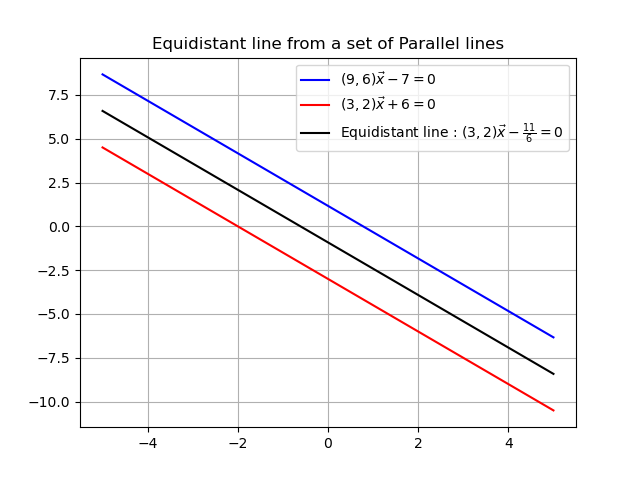
\includegraphics[width=\columnwidth]{graph.png}
 \caption{The equidistant line}
 \end{figure}
\end{document}
